%---------------------------------------------------------------------
%
%                          Cap�tulo 2
%
%---------------------------------------------------------------------
%
% 02EstructuraYGeneracion.tex
% Copyright 2009 Marco Antonio Gomez-Martin, Pedro Pablo Gomez-Martin
%
% This file belongs to the TeXiS manual, a LaTeX template for writting
% Thesis and other documents. The complete last TeXiS package can
% be obtained from http://gaia.fdi.ucm.es/projects/texis/
%
% Although the TeXiS template itself is distributed under the 
% conditions of the LaTeX Project Public License
% (http://www.latex-project.org/lppl.txt), the manual content
% uses the CC-BY-SA license that stays that you are free:
%
%    - to share & to copy, distribute and transmit the work
%    - to remix and to adapt the work
%
% under the following conditions:
%
%    - Attribution: you must attribute the work in the manner
%      specified by the author or licensor (but not in any way that
%      suggests that they endorse you or your use of the work).
%    - Share Alike: if you alter, transform, or build upon this
%      work, you may distribute the resulting work only under the
%      same, similar or a compatible license.
%
% The complete license is available in
% http://creativecommons.org/licenses/by-sa/3.0/legalcode
%
%---------------------------------------------------------------------

\chapter{Estado del arte en entrada de usuario para videojuegos}
\label{cap2}


A lo largo de las diferentes generaciones de computadores y de consolas se han ido desarrollando una serie de dispositivos de entrada que permiten al usuario interactuar con la m\'aquina. Estos dispositivos van desde teclados y ratones hasta c\'amaras que permiten transformar tus movimientos f\'isicos en movimientos dentro de un entorno virtual pasando por detectores de aceleraci\'on y pantallas t\'actiles. En este cap\'itulo se presentan muchos de los trabajos pasados en el \'ambito de los dispositivos de entrada de usuario.
%-------------------------------------------------------------------
\section{Breve introducci\'on a los dispositivos de entrada}

Los dispositivos de entrada son aquellos que permiten introducir datos o informaci\'on en un ordenador para que este los procese u ordene. Otro t\'ermino usado para estos dispositivos es perif\'erico. A pesar de que este t\'ermino implica a menudo el concepto de adicional y no esencial, en muchos sistemas inform\'aticos son elementos fundamentales. \cite{entradasalida} expone que los m\'as comunes de estos dispositivos de entrada son el teclado y rat\'on. Pero no existen \'unicamente estos 2 dispositivos de entrada, a lo largo de la historia de la inform\'atica se han ido desarrollando diversos dispositivos de entrada tanto sonora como visual y de movimiento mec\'anico.\\

\setcitestyle{super}

\subsection{Evoluci\'on de los teclados}

La historia de los teclados\cite{historiateclados} actuales tiene su origen en las m\'aquinas de escribir. Estas primeras m\'aquinas de escribir tienen su origen en el a\~no 1877, cuando la empresa Remington comenz\'o a comercializar de manera masiva las m\'aquinas de escribir. En un primer momento las teclas de dispusieron en orden alfab\'etico, algo que cambiar\'ia un a\~no despu\'es con la aparici\'on de la primera patente del teclado QWERTY. Tal y como se\~nala Jimmy Stamp\cite{jimmy} en su art\'iculo, esta primera versi\'on de las m\'aquinas de escribir ten\'ian un defecto que fue notorio cuando los usuarios escrib\'ian r\'apidamente una sucesi\'on de letras que se encontraban cerca en el teclado. Para evitar este fallo en el modelo inicial se desarroll\'o el sistema QWERTY, el cual distancia los pares de letras que se suelen escribir juntas.\\

Uno de los primeros avances de estas m\'aquinas de escribir ocurri\'o en la d\'ecada de 1930, cuando se combinaron la tecnolog\'ia de la entrada e impresi\'on de las m\'aquinas de escribir con la tecnolog\'ia de la comunicaci\'on del tel\'egrafo. Este dispositivo fue muy popular durante el siglo XX y sus funciones eran las de enviar y recibir mensajes mecanografiados de un punto a otro a trav\'es de un canal de comunicaci\'on. M\'as adelante fue utilizado en conjunto con las cintas perforadas para almacenar datos en los primeros ordenadores. As\'i, en 1955, el Whirlwind del MIT, se convierte en el primer ordenador del mundo que permite a sus usuarios introducir comandos a trav\'es de un teclado y confirma lo \'util y conveniente que puede ser un dispositivo de entrada como el teclado.\\

Actualmente las principales mejoras que han sufrido los teclados de ordenador se basan en la eliminaci\'on de cables gracias al Bluetooth. Con la llegada de los dispositivos t\'actiles se a\~nadi\'o adem\'as el concepto de teclado virtual. Este teclado virtual elimina el uso de un teclado hardware para pasar a un teclado software que imita el teclado tradicional QWERTY pero en una pantalla t\'actil. \\

\subsection{Evoluci\'on de los ratones}

Adem\'as del teclado, el segundo dispositivo de entrada por excelencia es el rat\'on. La primera maqueta fue dise\~nada durante los a\~nos 60, dispon\'ia de 2 ruedas met\'alicas que al desplazarse por una superficie mov\'ian 2 ejes. Cada uno de estos ejes controlaba el movimiento tanto vertical como horizontal del cursor en la pantalla y dispon\'ia de un bot\'on en la parte superior con el que se permit\'ia hacer clic en la posici\'on en la que se encontraba el cursor.\\

\begin{figure}[h]
\centering
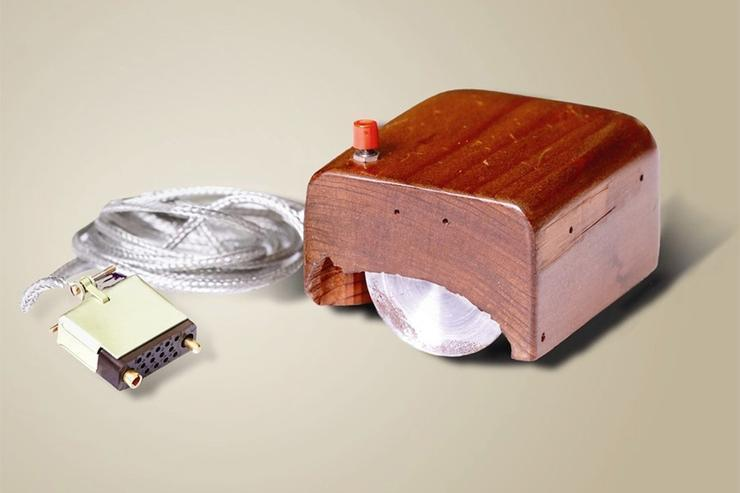
\includegraphics[width=0.29\textwidth]{./Imagenes/Bitmap/Primer_raton.jpg}
\caption{Primer rat\'on desarrollado por Douglas Engelbart y Bill English}
\label{Fig:primerraton}
\end{figure}

El siguiente avance del dispositivo fue cambiar su carcasa de madera por una de pl\'astico y a\~nadir m\'as botones. Tal y como describi\'o Daniel Entrialgo\cite{xerox} en su art\'iculo, este avance suele ser atribuido a Microsoft o a Apple pero fue la empresa \textbf{Xerox} la que realiz\'o el nuevo dise\~no del rat\'on y del que es considerado el primer ordenador personal de la historia junto al Altair 8080. Este nuevo dispositivo sustitu\'ia las 2 ruedas que marcaban la posici\'on del cursor por una \'unica bola de metal. La posici\'on relativa de esta bola era la que determinaba la posici\'on del cursor en la pantalla. 

\begin{figure}[!htb]
\begin{minipage}{0.9\textwidth}
    \centering
    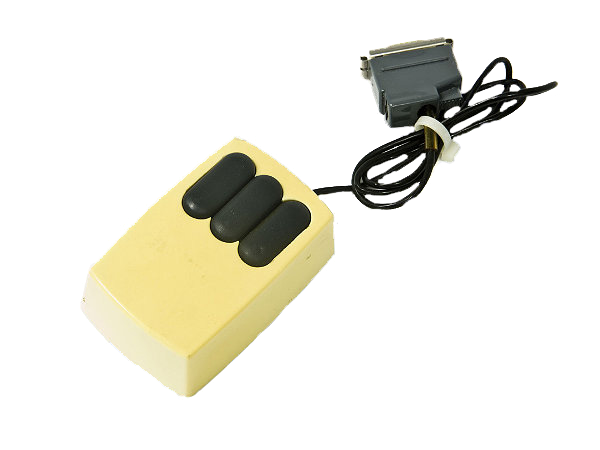
\includegraphics[width=0.40\textwidth]{./Imagenes/Bitmap/mouse_xerox_alto(1).png}
    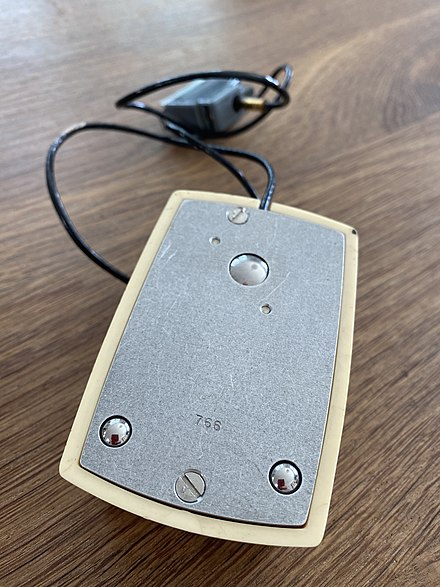
\includegraphics[width=0.20\textwidth]{./Imagenes/Bitmap/mouse_xerox_alto(2).jpg}
\end{minipage}
    \caption{Rat\'on del Xerox Alto de los a\~nos 70}
\label{Fig:xerox}
\end{figure}

En el a\~no 1992 Microsoft decidi\'o vender en un mismo paqueta su \'ultima versi\'on de MS-DOS y Windows 3.1, lo que hizo que el rat\'on pasase a ser un perif\'erico fundamental ya que se dejaba atr\'as el mundo del texto y se abr\'ian a todos los p\'ublicos las interfaces gr\'aficas del PC. Este cambio hizo que el rat\'on siguiera evolucionando y durante la d\'ecada de los 90 e inicios del 2000 los ratones sufrieron algunas mejoras. Algunas de estas mejoras son: una rueda central o lateral para el desplazamiento, el sensor de movimiento \'optico por diodo led o un sensor basado en un l\'aser no visible. Un sector que aprovech\'o mucho esta estandarizaci\'on del rat\'on y de las interfaces gr\'aficas fue el de los videojuegos. El rat\'on se ha convertido en una parte esencial del mundo de los videojuegos de PC, sirviendo no solo para seleccionar y accionar objetos en pantalla en juegos de estrategia, sino para controlar la c\'amara o cambiar la direcci\'on del personaje en juegos de primera y tercera persona.\\

\subsection{Evoluci\'on de los gamepads a trav\'es de las generaciones de consolas}

Los videojuegos de PC fueron, son y ser\'an muy importantes para el desarrollo de la industria pero las precursoras de este existo son sin dudas las m\'aquinas recreativas. Se dice que el primer intento de videojuego es una patente de 1947 sobre la simulaci\'on del lanzamiento de misiles pero no fue hasta 1958 y la salida del famoso ``Tenis para Dos''\cite{tenispara2} creado por William Higginbotham. En este juego se recreaba una pista de tenis en la que la pelota iba de un lado a otro de la pista. Poco despu\'es, en 


\subsubsection{Primera generaci\'on (1972-1976)}
a
\subsubsection{Segunda generaci\'on (1976-1983)}
a

\subsubsection{Tercera generaci\'on (1983-1987)}

a

\subsubsection{Cuarta generaci\'on (1987-1993)}


a

\subsubsection{Quinta generaci\'on (1993-1998)}

a

\subsubsection{Sexta generaci\'on (1998-2005)}

a


\subsubsection{Septa generaci\'on (2005-2012)}


a

\subsubsection{Octava generaci\'on (2012-2020)}

a

\subsubsection{Novena generaci\'on (2020-Actual)}
\subsection{Otros dispositivos}

Todos estos dispositivos de entrada son conocidos como \textbf{HID, Human Interface Device}. La principal motivaci\'on para HID era la de permitir innovaciones en los dispositivos de entrada a los ordenadores y as\'i simplificar el proceso de instalaci\'on de este tipo de dispositivos. Antes de HID, los dispositivos de entrada se ajustaban a unos estrictos protocolos dise\~nados para ratones, teclados y joysticks. Con cualquier innovaci\'on en el hardware se requer\'ia de sobrecargar el protocolo existente o la creaci\'on de un driver. Un solo driver HID analiza los datos de entrada y permite una asociaci\'on din\'amica de estos datos con la funcionalidad descrita por la aplicaci\'on. En el protocolo HID existen 2 enidades: el host y el dispositivo.El dispositivo es la entrada que intercat\'ua directamente con el humano, un ejemplo puede ser el teclado o rat\'on. El host es el que recibe los datos de entrada del dispositivo con las acciones ejecutadas por el humano, el host suele ser un ordenador.
 Los dispositivos definen sus paquetes de datos y luego presentan un descriptor HID al host. El descriptor HID es codificado como un grupo de bytes que describen los paquetes de datos del dispositivo. Esto incluye: cuantos paquetes soporta el dispositivo, el tama\~no de los paquetes, y el prop\'osito de cada byte y bit en el paquete. Se espera que el host sea la entidad m\'as compleja de las 2 ya que el host necesita obtener el descriptor HID del dispositivo y analizarlo antes de establecer la comunicaci\'on. El HID tambi\'en define el modo arranque, este modo es limitado ya que paquetes de datos son utilizados durante ese modo. Los \'unicos dispositivos que soportan el modo arranque son teclados y ratones.\\

En 1972 fue lanzada de manera oficial la \textbf{Magnavox Odyssey} y fue considerada la primera videoconsola. El dispositivo de entrada para poder jugar consit\'ia de 2 diales que se utilizaban para el movimiento horizontal y vertical del personaje, un cuadrado blanco. Como juego para la consola Odyssey sacaron el Magnavox Odyssey Shooting Gallery en 1972. El mando que se usaba para poder jugar a este juego tenía la forma de un rifle y la peculiaridad que tenía este accesorio/mando era que los disparos se registraban siempre y cuando el rifle apuntase a una luz intensa por lo que era muy f\'acil de enga\~nar si no fuese porque el juego no dispon\'ia de un registro de puntos. En 1976 la empresa Fairchild Semiconductor sac\'o al mercado la \textbf{Fairchild Channel F} cuya caracter\'istica principal a nivel de entrada de usuario fue la incorporaci\'on de un joystick de 8 direcciones.  Adem\'as de ofrecer un movimiento en 8 direcciones, la parte de arriba de este mando pod\'ia girarse para ser compatible con juegos como \textit{Pong} y tambi\'en pod\'ia ser pulsado y usarse normalmente como bot\'on de disparo. En 1977 sali\'o al mercado uno de los joysticks m\'as famosos. Este joystick es el que se utilizaba en la consola \textbf{Atari 2600}. Este joystick se conoc\'ia como el \textbf{Atari CX40} y consist\'ia de una palanca que permit\'ia un movimiento en 8 direcciones y un bot\'on. Junto con este modelo, Atari sac\'o al mercado un tipo de conexi\'on que se convertir\'ia en el est\'andar de la ind\'ustria y que ser\'ia compatible con sistemas posteriores. Unos pocos a\~nos despu\'es, en 1982, Atari lanz\'o su nueva consola Atari 5200. Adem\'as de mejorar gr\'aficamente, el controlador que llevaba incorporado proviene de un kit de controlador de un avi\'on RC. El sistema combinaba un dise\~no mec\'anico demasiado complejo con un sistema de circuito flexible interno de muy bajo coste. Este controlador incluy\'o un bot\'on de pausa, una caracter\'istica \'unica en ese momento.\\

En 1983 Nintendo sac\'o al mercado su \textbf{Nintendo Entertainment System (NES)} cuyo controlador sent\'o unas bases en el control del movimiento gracias a la cruceta que incorporaba. Esta cruceta permit\'ia un movimiento en 4 direcciones y que pretend\'ia reemplazar a las voluminosas palancas de mando de los controladores. Adem\'as de la cruceta, el mando dispon\'ia de 2 botones redondos (A y B) y otros 2 botones rectangulares (START y SELECT). En lo sucesivo, se lanzaron varios dispositivos especiales dise\~nados precisamente para usarse con juegos espec\'ificos, aunque muy pocos de estos se volvieron populares. Uno de estos dispositivos era el \textbf{Power Glove}, el que ser\'ia considerado como uno de los primeros perif\'ericos de interfaz en recrear los movimientos de la mano en una pantalla de televisi\'on o de un ordenador en tiempo real. En 1990 Nintendo hizo evolucionar a la Nintendo NES y lanz\'o la \textbf{Super Nintendo Entertainment System (SNES)}, la cual dej\'o atr\'as un dise\~no cuadrado del controlador y se inclin\'o por un dise\~no m\'as ergon\'omico, se mejor\'o la cruceta y se a\~nadieron otr\'os 2 botones (X e Y). El tiempo de respuesta del controlador era de 16 milisegundos. Dentro de la evoluci\'on de los controladores, en 1993 la compa\~nia SEGA sorprendi\'o con el lanzamiento de un nuevo accesorio para su consola \textbf{Sega Mega Drive}. Este accesorio consist\'ia en un aro octogonal que se colocaba en el sueloy se conectaba directamente al puerto de controlador de la consola. Lo llamaron \textbf{Sega Activator} y fue el primer controlador que utilizaba el cuerpo completo. El jugador se ten\'ia que situar en el centro del aro, el cual emit\'ia rayos infrarrojos hacia arriba para detectar los movimientos del jugador. Los juegos orientados para el Sega Activator eran juegos que involucrasen el movimiento de brazos y piernas para que el jugador cruzase los rayoss infrarrojos y as\'i se detectase el movimiento. Al tratarse de 8 segmentos, cada uno de estos segmentos estaba mapeado como si fuera un bot\'on en el mando tradicional, el cual se "pulsar\'ia" cada vez que el jugador cruzase un segmento de los rayos infrarrojos. \\

Durante los a\~nos 90 \textbf{Sony} entr\'o al terreno del desarrollo de consolas y por consecuencia, de modelos diferentes de controladores de videojuegos. Con su primera consola, la \textbf{Sony PlayStation}, incluyeron un nuevo dise\~no de mando que recog\'ia muchos de los dise\~nos vistos hasta el momento. A diferencia de Nintendo, este controlador cambi\'o la nomenclatura de los botones A,B,Y y X por las figuras $\triangle$, O, X y $\Box$, manten\'ia la cruceta y los botones START y SELECT y adem\'as a\~nadi\'o 4 botones m\'as en la parte lateral del mando para los dedos \'indice y coraz\'on. 3a\~nos m\'as tarde Sony sacar\'ia una re-edici\'on del mando al que le incorporaron 2 stickts anal\'ogicos junto con un bot\'on con un LED para cambiar entre los diferentes modos usados para el control del personaje. Este modelo fue el predecesor del famoso \textbf{DualShock} y \'unicamente la versi\'on japonesa presentaba una funci\'on de retroalimentaci\'on de vibraci\'on. Por el lado de Nintendo, la consola sucesora de la Super Nintendo fue la \textbf{Nintendo 64} que fue acompa\~nada por un nuevo dise\~no de mando que no pas\'o desapercibido. Dispon\'ia de una cruceta en la parte izquierda del mando, un stick de 360 grados y un bot\'on START en el centro del mando y 6 botones en su parte derecha. Complementario a esto, en la parte trasera del mando hab\'ia 2 botones m\'as y tambi\'en en la parte trasera se daba la opci\'on de introducir un dispositivo extraible que proporcionaba retroalimentaci\'on de vibraci\'on. Este accesorio se activaba en ocasiones concretas como al disparar un arma y serv\'ia para sumergir al jugador en el videojuego.\\

En los a\~nos posteriores las compa\~nias siguieron sacando modelos direferentes mandos que modificaban tama\~no y posiciones de los botones pero no salieron cambios significativos hasta que en 2002 Nintendo lanz\'o al mercado un nuevo mando alternativo para su consola \textbf{GameCube}, este controlador ten\'ia la peculiaridad de ser inal\'ambrico. Lo llamaron \textbf{WaveBird Wireless Controller} y sent\'o las bases para los pr\'oximos mandos inal\'ambricos. Contaba con una cruceta, 6 botones digitales, 2 botones h\'ibridos ya que hacian la funci\'on de gatillos y 2 palancas anal\'ogicas para el movimiento del personaje y la c\'amara normalmente. Como alimentaci\'on usaba 2 pilas AA y para comunicarse con la consola usaba radiofrecuencia, lo que permit\'ia al jugador alejarse hasta 6 metros de la consola. Poco tiempo despu\'es tanto Sony con su PlayStation 3 como Microsoft con su Xbox 360 a\~nadir\'ian las baterias a sus mandos para convertirlos en inal\'ambricos. \\

En 2006 Nintendo  volvi\'o a sorprender a la sociedad con la llegada de la \textbf{Nintendo Wii} y su nuevo mando. \textbf{Nintendo Wiimote} es el mando principal de la consola Wii y las caracter\'isticas destacables que trae son la de la detecci\'on de movimiento en el espacio y la habilidad de poder apuntar a objetos en la pantalla. El dise\~no del mando de Wii deja de lado todos los modelos tradicionales de mandos para videojuegos y se acerca m\'as a un control remoto de televisi\'on para que este pueda usarse con una sola mano y sea m\'as intuitivo ya que lo que pretend\'ia era cautivar a un p\'ublico m\'as casual y ser una consola para todos los miembros de la familia. En la cara frontal del mando se encuentran los botones ``A'', ``1'', ``2'', ``+'', ``-'', ``HOME'' y la cruceta, m\'as un bot\'on ``POWER'' para apagar la consola, algo in\'edito hasta entonces. En la parte anterior s\'olo presenta el bot\'on ``B'', en un formato similar a un gatillo. Adem\'as de los botones, en la parte frontal lleva incorporado un altavoz y 4 luces numeradas que indican el j\'umero de jugador al que corresponde cada mando durante una partida. Lleva una correa de seguridad udia al mando por laparte inferior de este para poder atar el mando a la mu\~neca y evitar asi que el mando se resbale durante una sesi\'on de juego y o el mando o la televisi\'on se vieran da\~nados. El Wii Remote tiene la capacidad de detectar la aceleraci\'on a lo largo de tres ejes mediante la utilizaci\'on de un aceler\'ometro. El Wiimote tambi\'en cuenta con un sensor \'optico PixArt, lo que le permite determinar el lugar al que el Wiimote est\'a apuntando; adem\'as de agregar una br\'ujula electr\'onica en su posterior versi\'on mejorada, el \textbf{WiiMotionPlus.} A diferencia de controladores que detectan la luz de la pantalla del televisor, el Wii Remote detecta la luz de una barra sensor que ven\'ia incorporada con la consola y se colocaba encima de la pantalla. No es necesario se\~nalar directamente a la barra sensor, pero apuntar significativamente fuera de la barra de posici\'on perturbar\'a la capacidad de detecci\'on debido al limitado \'angulo de visi\'on del Wiimote. La posici\'on y seguimiento del movimiento del Wii Remote permite al jugador imitar las acciones reales de juego, como blandir una espada o una pistola con objetivo, en lugar de simplemente pulsando los botones. El Wii Remote tiene incorporado un altavoz que emite sonidos diferentes que los emitidos por lo altavoces de la televisi\'on y que se utilizan para mejorar la ambientaci\'on del videojuego. El ejemplo de esto se mostr\'o en el E3 de 2006 cuando uno de los desarrolladores dispar\'o un arco en ``The Legend of Zelda: Twilight Princess'' y por el mando son\'o como tensaba y soltaba la flecha mientras que en la televisi\'on \'unicamente se escuchaba el impacto de la flecha. Esto daba la sensaci\'on de que la flecha viajaba desde el jugador hasta la televisi\'on. Esto se ve\'ia acompa\~nado por la vibraci\'on del mando y ambas funciones pod\'ian deshabilitarse desde el men\'u HOME de la consola, en ese caso todos los sonidos saldr\'ian por los altavoces de la televisi\'on. En cuanto a la duraci\'on de las baterias, con las funciones m\'as b\'asicas de algunos juegos ten\'ia la autonom\'ia de 60 horas y en caso de usar todas sus capacidades llegaba a aguantar 25 horas funcionando. Al tratarse de un mando sim\'etrico su uso estaba pensado tanto para zurdos como para diestros y se utilizaba tanto de manera vertical con una sola mano como de manera horizontal en caso de usar ambas manos. Adem\'as de todo lo anterior, en la parte inferior del mando se encuentra un puerto de expansi\'on para conectar diferentes perif\'ericos. Los m\'as usado fueron el \textbf{Wii Balance Board} que se trataba de una tabla capaz de calcular la presi\'on que se ejerc\'ia sobre ella, el \textbf{Wii Guitar} que permit\'ia jugar al juego Guitar Hero en su versi\'on de Wii, \textbf{Nunchuck} que agregaba un joystick anal\'ogico y 2 botones m\'as para el movimiento de personajes, \textbf{Wii Wheel} que hac\'ia que el Wii Remote se convirtiese en un volante y asi poder tener una mejor experiencia en juegos como Mario Kart y \textbf{Wii MotionPlus} que incorporaba 3 sensores nuevos de movimiento para los ejes vertical, longitudinal y lateral lo que ayud\'o a mejorar la precisi\'on del mando original.\\

En 2010 Microsoft dio el salto a un nuevo controlador de videojuegos para su consola Xbox 360. Este nuevo perif\'erico es conocido con el nombre de \textbf{Kinect} y permite a los usuarios controlar e interactuar con la consola sin necesidad de tener contacto f\'isico con un mando tradicional. Este control se realiza por gestos y reconocimiento de voz. El sensor Kinect es una barra horizontal de unas 9 pulgadas conectada a una peque\~na base circular con un eje que permiteque esta rote y adem\'as est\'a dise\~nado para ser colocado por encima o por debajo de la televisi\'on. El dispositivo cuenta con una c\'amara RGB, un sensor de profundidad, un micr\'ofono de m\'ultiples matrices y un procesador personalizado que ejecuta el software patentado, que proporciona captura de movimiento de todo el cuerpo en 3D, reconocimiento facial y capacidades de reconocimiento de voz. El micr\'ofono de matrices del sensor de Kinect permite a la Xbox 360 llevar a cabo la localizaci\'on de la fuente ac\'ustica y la supresi\'on del ruido ambiente, permitiendo participar en el chat de Xbox Live sin utilizar auriculares. El sensor de profundidad es un proyector de infrarrojos combinado con un sensor CMOS monocromo que permite a Kinect ver la habitaci\'on en 3D en cualquier condici\'on de luz ambiental. El rango de detecci\'on de la profundidad del sensor es ajustable gracias al software de Kinect capaz de calibrar autom\'aticamente el sensor, basado en la jugabilidad y en el ambiente f\'isico del jugador, tal como la presencia de sof\'as, mesas y otro tipo de muebles.\\

PlayStation tambi\'en lanz\'o al mercado su dispositivo de control de videojuegos por movimiento, ellos lo llamaron \textbf{PlayStation Move} y es compatible con los sitemas PS3 y PS4. PlayStation Move compiti\'o tanto con el Kinect de Xbox como con el WiiMote de Nintendo. El dise\~no del mando consiste en un mando similar al de Wii ya que ambos se controlar con una mano en vertical. PlayStation Move uni\'o los conceptos de sensores de movimiento que usaba el WiiMote y la c\'amara que usaba el Kinect, por lo que PlayStation Move usa sensores de movimiento en el mando,una esfera en su extremo que se ilumina y la c\'amara PlayStation Eye que detecta la posici\'on del mando.Al igual que en el resto de controladores inal\'ambricos para PlayStation, tanto el mando principal de PlayStation Move como el Navigation Controller usan la conexi\'on inal\'ambrica Bluetooth 2.0 y una bater\'ia de ion de litio, que se carga mediante un puerto USB Mini-B. El Naigation Controller es un mando que complementa al mando principal y tiene una funci\'on similar a la del Nunchuck de Wii. Se pueden conectar hasta 4 PlayStation Move de manera simult\'anea.\\
 
Coincidiendo con la salida al mercado del PlayStation Move, Nintendo lanz\'o su nueva consola en 2012; la \textbf{Wii U} y con ella un Controlador de videojuegos h\'ibrido. Este controlador h\'ibrido es el \textbf{Wii U GamePad} y es el mando principal de la consola. La principal distinci\'on con respecto a los mandos tradicionales es la incorporaci\'on de una pantalla t\'actil, la cual se utiliza para mostrar informaci\'on adicional durante una partida y adem\'as puede usarse como pantalla principal en caso de no disponer de un televisor mientras se juega. Adem\'as de como controlador de videojuegos, el Wii U GamePad es utilizado como control remoto independiente para cotrolar la pantalla de la televisi\'on u otro aparato via infrarrojos sin tener que tener la consola encendida. El mando constaba de altavoces y micr\'ofono e incorporaba una c\'amara frontal de 1.3 megapixeles. Los sensores que incorporaba eran: aceler\'ometro, giroscopio, geomagn\'etico e infrarrojo e incorporaba vibraci\'on. La conexi\'on a la consola se hac\'ia mediante bluetooth  y dispon\'ia de NFC para futuros accesorios que incorporaron a los diferentes videojuegos.\\

En 2013 Sony hizo una revisi\'on de su DualShock y como mando de la consola PlayStation 4 lanz\'o el \textbf{DualShock 4}. Este mando a\~nadi\'o al dise\~no anterior una pantalla t\'actil en la parte frontal, lo que hizo que la distribuci\'on de los botones que antes eran centrales cambiasen. En la parte trasera se a\~nadi\'o una barra LED que se ilumina en varios colores para diferenciar e identificar a los diferentes jugadores. Microsoft por su parte en 2015 puso a la venta su nuevo \textbf{Xbox One Elite Controller}. Una de las principales caracter\'isticas es que tiene un dise\~no modular por lo que cada pieza es intercambiable para que cada jugador pueda adaptarlo a su medida. La personalizaci\'on es el principal aliciente en este mando ya que permite reprogramar tanto los cuatro botones tradicionales de la parte frontal como los gatillos. Tambi\'en se da la posibilidad de establecer curvas de sensibilidad en las palancas anal\'ogicas. Gracias a la posibilidad de a\~nadir piezas, este mando incluye 4 palancas m\'as en la parte trasera.\\

En 2017 Nintendo present\'o su nueva consola h\'ibrida que se basa en su predecesora, Wii U. La consola es \textbf{Nintendo Switch} y es una consola que puede ser jugada tanto de manera port\'atil como de sobremesa en una televisi\'on o un monitor. Loa mando dise\~nados para esta consola son los \textbf{Joy Con} y consisten en 2 unidades, cada uno de ellos contiene una palanca anal\'ogica y una matriz de botones. Estos mandos tienen la peculiaridad de que pueden usarse tanto acoplados a la consola cuando esta se utilice en modo port\'atil o pueden ser desacoplados para cuando la consola se utilice en una televisi\'on. Cuando se separan, un par de Joy-Con pueden ser utilizados por un solo jugador, o dividido entre dos como controladores individuales. Los Joy-Con se distribuyen en pares, designados como ``Joy-Con L'' y ``Joy-Con R'', respectivamente. Este dise\~no viene heredado de Wii con su Wiimote y el accesorio principal el Nunchuk. Una misma Nintendo Switch puede tener conectados hasta un total de 8 Joy-Con. La comunicaci\'on que tienen con la consola se realiza por Bluetooth y disponen de una correa igual a la del mando de Wii para evitar la caida del mando durante su uso. Los Joy-Con contienen bater\'ias no extraibles de 525 mAh, que se cargan cada vez que se conectan a la consola. Ambos controladores contienen una palanca anal\'ogica, cuatro botones de cara, dos botones superiores, dos botones laterales accesibles cuando se sueltan y designados como SL y SR, un bot\'on ``+'' o ``-'', un bot\'on de sincronizaci\'on y un indicador de jugador luces LED. Cada uno de los Joy-Con contiene un aceler\'ometro y un giroscopio, que pueden ser utilizados para los juegos que incluyen movimiento. La diferencia con el mando de Wii es que estos mandos no necesitan una barra de sensores para su correcto funcionamiento. Adem\'as, el Joy-Con R contiene un sensor de seguimiento de profundidad infrarroja, que puede leer objetos y movimientos sostenidos delante de \'el. Cada uno de los Joy-Con incorpora un motor para la vibraci\'on del mando durante las sesiones de juego. Poco despu\'es de su salida, se descubri\'o que los Joy-Con pueden conectarse y utilizarse con otros ordenadores personales y con dispositivos m\'oviles a trav\'es de la conexi\'on Bluetooth.\\

Tambi\'en durante 2017, Sony anunci\'o una serie de juegos nuevos que se jugar\'ian de una forma totalmente diferente ya que el mando utilizado ser\'ia cada uno de los tel\'efonos m\'oviles de los usuarios. A esta serie de juegos se la conoce como \textbf{PlayLink}. La idea detr\'as de PlayLink es que todos los usuarios de la consola PlayStation 4 y sus familiares y amigos disponen de un dispositivo m\'ovil pero no todos disponen de varios mandos para poder jugar con m\'as personas en juegos cooperativos. PlayLink es una aplicaci\'on m\'ovil que cada usuario se descarga en su Android o iOS y as\'i puede usar su tel\'efono como un mando m\'as de PlayStation 4. El requisito para que la conexi\'on sea efectiva es que tanto la consola PS4 como los dispositivos m\'oviles que se vayan a usar est\'en conectados a la misma red WIFI.\\

A finales del a\~no 2020 Sony lanz\'o al mercado su nueva consola, la PS5 y con ella un nuevo mando al que bautizaron como \textbf{DualSense}. Como ya pasaba con el DualShock 4, este mando funciona con bater\'ia y lleva un altavoz integrado. Adem\'as de esto, el DualSense incorpora un aceler\'ometro y un giroscopio para aquellos juegos compatibles con esta tecnolog\'ia. La gran novedad que trae este mando es la retroalimentaci\'on h\'aptica. Se han sustituido los motores de vibraci\'on tradicionales por 2 activadores que emiten vibraciones din\'amicas capaces de simular todo tipo de sensaciones. Adem\'as de la nueva retroalimentaci\'on h\'aptica, el nuevo DualSense incorpora 2 gatillos adaptativos. Estos gatillos emiten diferente fuerza de resistencia contra el jugador dependiendo del arma que se est\'e utilizando. El ejemplo que pusieron los desarrolladores de Sony fue con la cuerda de un arco, inicialmente no tiene resistencia pero cuanto m\'as se tense la cuerda del arco m\'as fuerza es necesaria.

\section{\textit{Feedback} en los controladores}

En los inicios de los videojuegos y de las consolas el objetivo fue la creaci\'on de nuevos tipos de juegos con diferentes mec\'anicas y mejoras gr\'aficas. En la era actual de los videojuegos se ha ido mucho m\'as lejos de los primeros juegos como Pong y Tetris, la tendencia ha llevado a la creaci\'on de escenarios virtuales m\'as realistas y a que el jugador formase parte de ese entorno virtual. Particularmente la respuesta que se da al usuario del videojuego al realizar acciones es conocida como \textbf{tecnolog\'ia h\'aptica}. Este tipo de tecnolog\'ia se refiere al conjunto de interfaces tecnol\'ogicos que interaccionan con una persona mediante el sentido del tacto. La tecnolog\'ia h\'aptica tiene sus inicios en los dispositivos de los sistemas servo para controlar grandes aviones con la intenci\'on de poder hacerlo de manera remota. En estos sistemas se instal\'o un sistema de control que proporcionaba una resistencia a la palanca del piloto proporcional al \'angulo de ataque del avi\'on. Otro ejemplo destacable de esta tecnolog\'ia se encuentra en la pel\'icula \textbf{4-D Honey, I Shrunk the Audience!} del a\~no 1994 que simulaba que los ratones se soltaban por el auditorio y corrian por toda la sala. Para conseguir esta simulaci\'on se bombeaba aire a trav\'es de un peque\~no tubo de pl\'astico y al agitarse, imitaba la sensaci\'on de las colas de los ratones rozando las piernas de los espectadores. \\

En los videojuegos esta tecnolog\'ia fue introducida a trav\'es de los controladores. Al inicio estos sistemas de vibraci\'on se introdujeron en los controladores como dispositivos que se acomplaban al mando por separado pero con la salida de la versi\'on japonesa del controlador de PlayStation, el Dualshock. Este mando incorporaba un sistema de vibraci\'on conocido como \textit{tabletas vibradoras (rumble packs)} que ten\'ian ese efecto de vibraci\'on al conducir veh\'iculos o disparar armas de fuego. Con la llegada de las pantallas t\'actiles tambi\'en aparecieron las pantallas h\'apticas. Estas pantallas son aquellas que transmiten una vibraci\'on al tocarla. El ejemplo m\'as actual de tecnolog\'ia h\'aptica puede encontrarse en la reciente consola de Nintendo, Nintendo Switch. Nintendo no ha denominado a la tecnolog\'ia que usan sus Joy-Cons como tecnolog\'ia h\'aptica sino como \textbf{Rumble HD} pero Nintendo se ha asegurado en demostrar todas las capacidades que sus nuevos Joy-Cons pueden ofrecer en cuanto a este tipo de tecnolog\'ia. Con su juego 1-2 Switch recogen una serie de minijuegos que tienen como objetivo el de mostrar las capacidades de los nuevos controladores, los Joy-Con. Entre estos minijuegos se encuentra uno en el que el jugador tiene que agitar el Joy-Con que simula un vaso con hielos y tiene que averiguar cu\'antos hielos hay en el vaso. Microsoft por su parte a\~nadi\'o a sus controladores de la consola Xbox One 4 motores de vibraci\'on que daban una mejor experiencia a los usuarios cuando estos conduc\'ian, disparaban armas de fuego o produc\'ian explosiones. Sony, por su parte, ha introducido un nuevo modelo de mando al que ha llamado \textbf{DualSense} para su nueva consola \textbf{PlayStation 5}. Con este mando Sony ha dejado atr\'as la vibraci\'on tradicional de los motores que llevaban incorporados los DualShock 4 y han introducido una retroalimentaci\'on h\'aptica mucho m\'as definida y precisa. Esta tecnolog\'ia recuerda al Rumbre HD que Nintendo incorpor\'o en sus Joy-Con pero en este caso siguiendo la est\'etica de los mandos tradicionales de Sony. Para complementar este \textit{feedback}, el DualSense incorpora 2 gatillos adaptativos que ofrecen diferentes niveles de resistencia. Esto permite al mando simular efectos de dentro del juego directamente en las manos del jugador como la tensi\'on de un arco al disparar una flecha o la diferencia entre disparar una escopeta y una ametralladora. Sony ha incluido con la consola el juego \textbf{Astro's Playroom} en el que con una serie de niveles y minijuegos se explotan al m\'aximo las nuevas caracter\'isticas que trae el nuevo DualSense a la PlayStation 5.


\section{Sistemas de \textit{streaming}}

Una transmisi\'on en directo consiste en una distribuci\'on digital de contenido multimedia a trav\'es de una red de ordenadores de manera que el usuario consume el producto a la vez que se descarga. El t\'ermino \textit{retransmisi\'on} se refiere a una corriente continua que fluye sin interrupciones, normalmente la difusi\'on es de audio o v\'ideo. Para referirse a una retransmisi\'on se suele utilizar el anglicismo \textit{streaming}. Esta tecnolog\'ia funciona gracias a un b\'ufer de datos que almacena el flujo de descarga en la estaci\'on del usuario e inmediatamente mostrar el material descargado. En contraposici\'on a esto se encuntra la descarga de archivos completos que requiere que el usuario descargue los archivos necesarios al completo para poder acceder al contenido. En el a\~no 1993 se consigui\'o que el grupo de m\'usica \textit{Severe Tire Damage} actuase en directo a trav\'es de Internet. Este concierto tuvo lugar en California y pudo verse hasta en Australia gracias a la tecnolog\'ia \textbf{Mbone}. Mbone es la abreviatura que se dio a \textit{Multicast backbone (Red troncal de multidifisi\'on)} y consist\'ia en una red troncal experimental y una red virtual que se contruy\'o sobre internet para el transportal el tr\'afico de la multidifusi\'on de IPs. Dado que los operadores de la mayor\'ia de los enrutadores de Internet ten\'ian deshabilitado la multidifusi\'on IP debido a preocupaciones relacionadas con el seguimiento del ancho de banda y la facturaci\'on, Mbone fue creado para conectar redes con capacidad de multidifusi\'on a trav\'es de la infraestructura de Internet existente en el momento. El prop\'osito principal de Mbone era el de minimizar la cantidad de datos requeridos para realizar una videoconferencia a diferentes puntos simult\'aneamente. Algunas de las caracter\'isticas de Mbone son:\par

\begin{itemize}
\item El protocolo de enrutado de multidifusi\'on utilizado fue \textbf{DVMRP (Distance Vector Multicast Routing Protocol)}. El funcionamiento de este protocolo consiste en la recepci\'on de paquetes a un router y si este proviene de un camino que podr\'ia utilizarse para alcanzar al emisor del mensaje original, este paquete se difunde por todos los dem\'as caminos activos. En caso contrario se elimina el paquete. 
\item La IP utilizada por Mbone fue 224.2.0.0 
\item Los requisitos de banda ancha para la transmisi\'on de audio eran 32-64 kbits/s y para video 120 kbits/s.
\end{itemize}

En 1994 el grupo brit\'anico \textit{The Rolling Stones} decidi\'o retransmitir en directo y de forma gratuita 20 minutos de uno de sus conciertos. Con el paso de los a\~nos empresas como QuickTime, ActivePlayer,Adobe, etc siguieron realizando experimentos para mejorar esta tecnolog\'ia. Solamente faltaba que las conexiones a internet a nivel global mejoraran. \par

Otro hito destacable en esta evoluci\'on fue el streaming ejecutado por Justin Kan, fundador de Justin.tv, ajustando una c\'amara web a su gorra y personalizando su port\'atil en su maleta para transmitir 24 horas durante los 7 d\'ias de la semana su vida cotidiana. M\'as adelante la compa\~nia creada por Justin se transformar\'ia en la famosa plataforma de streaming \textbf{Twitch.tv} que en el a\~no 2019 alcanz\'o un pico de 982 millones de espectadores simult\'aneos en los diversos canales que emiten en la plataforma. Para poder proporcionar un acceso claro, convincente, continuo y sin interrupciones ni cambios, la retransmisi\'on se apoya en las siguientes tecnolog\'ias:
\begin{itemize}
\item \textbf{C\'odecs}: C\'odec es el acr\'onimo de codificador-decodificador. Sirven para codificar el flujo o la se\~nal y recuperarlo o descifrarlo para la reproducci\'on en un formato adecuado para estas operaciones. Algunos c\'odecs son MP3, formato de compresi\'on de audio digital un algor\'itmo de p\'erdida para conseguir un menor tama\~no de archivo. Para video se suele usar el c\'odec H.264, el usado por la plataforma \textit{Youtube} para la visulaizaci\'on de sus videos y directos.
\item \textbf{Secuencia de bits}: Las emisiones de audio y v\'ideo en c\'odecs se ensamblan en un contenedor de secuencia de bits como \textbf{FLV (Flash Video)}. FLV fue ampliamente utilizado para transmitir v\'ideo por Internet sobre el complemento Adobe Flash Player. Flash Video puede ser visto en la mayor\'ia de los sistemas operativos mediante el plugin Adobe Flash Player, disponible para la mayor\'ia de navegadores web o de otros programas de terceros.
\item \textbf{Protocolos de transporte} : El uso de protocolos de transporte ligeros como \textbf{UDP} o \textbf{RTSP (Real Time Spread Protocol)} es algo que se busca en la retrasnmisi\'on de informaci\'on para que el ancho de banda a usar sea menor. UDP y RTSP hacen que las entregas de paquetes de datos desde el servidor a quien reproduce el archivo se hagan con una velocidad mucho mayor que la que se obtiene por \textbf{TCP} y \textbf{HTTP}. Esta eficiencia es alcanzada por una modalidad que favorece el flujo continuo de paquetes de datos. Cuando TCP y HTTP sufren un error de transmisi\'on, siguen intentando transmitir los paquetes de datos perdidos hasta conseguir una confirmaci\'on de que la informaci\'on lleg\'o en su totalidad. Sin embargo, UDP contin\'ua mandando los datos sin tomar en cuenta interrupciones, ya que en una aplicaci\'on multimedia estas p\'erdidas son casi imperceptibles. Aunque UDP no haga un control de transmisi\'on, la aplicaci\'on que use este protocolo para la retransmisi\'on tendr\'a que ser la encargada de realizarlo para tomar decisiones sobre qu\'e hacer ante un posible extrav\'io de informaci\'on.
\item \textbf{Ancho de banda}: Los anchos de banda recomendados para cada una las resoluciones incrementa de manera directamente proporcional con la calidad a la que se reproduce el contenido. Para la transmisi\'on de un v\'ideo en defini\'on est\'andar como la usada por Google TV, los discos Blue-Ray o Apple TV es de 2 Mbit/s. En caso de querer aumentar la calidad a alta deficini\'on se piden 5 Mbit/s y para el contenido con definici\'on ultra se piden 9 Mbit/s. Si el archivo se almacena en un servidor para transmisi\'on bajo demanda y 1000 personas ven este flujo al mismo tiempo usando un protocolo Unicast, el requisito es 300 kbit/s x 1000 = 300000 kbit/s = 300 Mbit/s de banda ancha. Esto equivale a alrededor de 135 GB por hora. Usando un protocolo de multidifusi\'on, el servidor env\'ia una sola transmisi\'on que es com\'un a todos los usuarios. Por lo tanto, dicha transmisi\'on solo usar\'ia 300 kbit/s de ancho de banda de servicio.  El c\'alculo para la transmisi\'on en vivo es similar. Suponiendo que la semilla en el codificador es de 500 kbit/s y si la emisi\'on dura 3 horas con 3000 espectadores, los c\'alculos ser\'ian (500 kbit/s x (3 x 3600) segundos x 3000 personas) / (8 x 1024 x 1024) lo que da un resultado de 1,977,539 MB consumidos para la visualizaci\'on de un directo por 3000 personas con un ancho de banda de 500kbit/s.
\end{itemize}

En Espa\~na los servicios de retransmisi\'on son populares entre la poblaci\'on y un estudio realizado por el Ministerio de Cultura de Espa\~na durante los a\~nos 2018-2019 realiz\'o una encuenta a 16000 personas sobre si se hac\'ian descargas ilegales de contenidos o si por el contrario estaban suscritos a servicios con suscripci\'on como Amazon Prime Video, Spotify, Netflix, etc. 
\begin{table}[H]

\begin{tabularx}{0.8\textwidth} { 
  | >{\raggedright\arraybackslash}X 
  | >{\centering\arraybackslash}X 
  | >{\raggedleft\arraybackslash}X | }
 \hline
 \textbf{Plataformas} & \textbf{\%} \\
 \hline
Pel\'iculas y series  & 38.9 \%  \\
\hline
TV  & 28.8 \%  \\
\hline
M\'usica  & 26.8 \%  \\
\hline
Libros  & 3.4 \%  \\
\hline
Videojuegos  & 4.1 \%  \\
\hline
\end{tabularx}
\caption{Porcentaje de suscripciones totales a plataformas digitales en Espa\~na en 2018-2019}
% referencia http://www.culturaydeporte.gob.es/servicios-al-ciudadano/estadisticas/cultura/mc/ehc/2018-2019/presentacion.html
\label{table:1}
\end{table}%

La conclusi\'on final fue que el 52.2\% de los usuarios encuestados ten\'ia una suscripci\'on activa a alguna plataforma digital.

%-------------------------------------------------------------------


% Variable local para emacs, para  que encuentre el fichero maestro de
% compilaci�n y funcionen mejor algunas teclas r�pidas de AucTeX
%%%
%%% Local Variables:
%%% mode: latex
%%% TeX-master: "../ManualTeXiS.tex"
%%% End:
